\section{Additional Experiment Analysis}
\label{appendix:additional-analysis}


\subsection{Additional Analysis on \ours}
\label{appendix::more-experiments}

\begin{wraptable}{r}{0.6\textwidth}
    \centering
    \begin{tabular}{l|c|c|c}
        \toprule
        Methods & Long & Multi-Hop & Simple \\
        \midrule
        \midrule
        \ours & 57.04\% & 74.22\% & 76.67\% \\
        \quad-w/o CS & 51.01\% & 74.22\% & 73.07\% \\
        \midrule
        HippoRag2 \cite{Main6} & 38.06\% & 68.04\% & 73.08\% \\
        \bottomrule
    \end{tabular}
    \caption{Ablation Study (Accuracy $\uparrow$). "CS" denotes the Contextual Skeleton Network in the Knowledge Graph. Using "GPT-4o-mini" as the backbone.}
    \label{tab:ablation-study}
\end{wraptable}

 % \add{what is contextual connections}
\textbf{Contextual Information Capture Capability.} We designed ablation experiments to investigate the impact of Contextual Skeleton Network in \ours's knowledge graph variants on performance, with results shown in \Cref{tab:ablation-study}. The experimental results demonstrate that removing the Contextual Skeleton Network leads to a slight performance degradation in \ours~ (no effect was observed in Multi-Hop question scenarios since the input data inherently consists of discrete single documents without multi-chunk cases within individual documents). Through in-depth analysis, we identify that this performance decline may stem from the following mechanism: The token-based chunking strategy may forcibly segment semantically coherent text, thereby compromising textual integrity. For instance, when the referent entity in a text fragment appears as a pronoun, the knowledge graph typically fails to establish direct associations between this entity and the text fragment. In contrast, large language models (LLMs) can actively access relevant contextual information through the chain connections of the Contextual Skeleton Network, thereby compensating for this deficiency.

\begin{figure}[htbp]
    \centering
    \begin{subfigure}[b]{0.48\textwidth}
        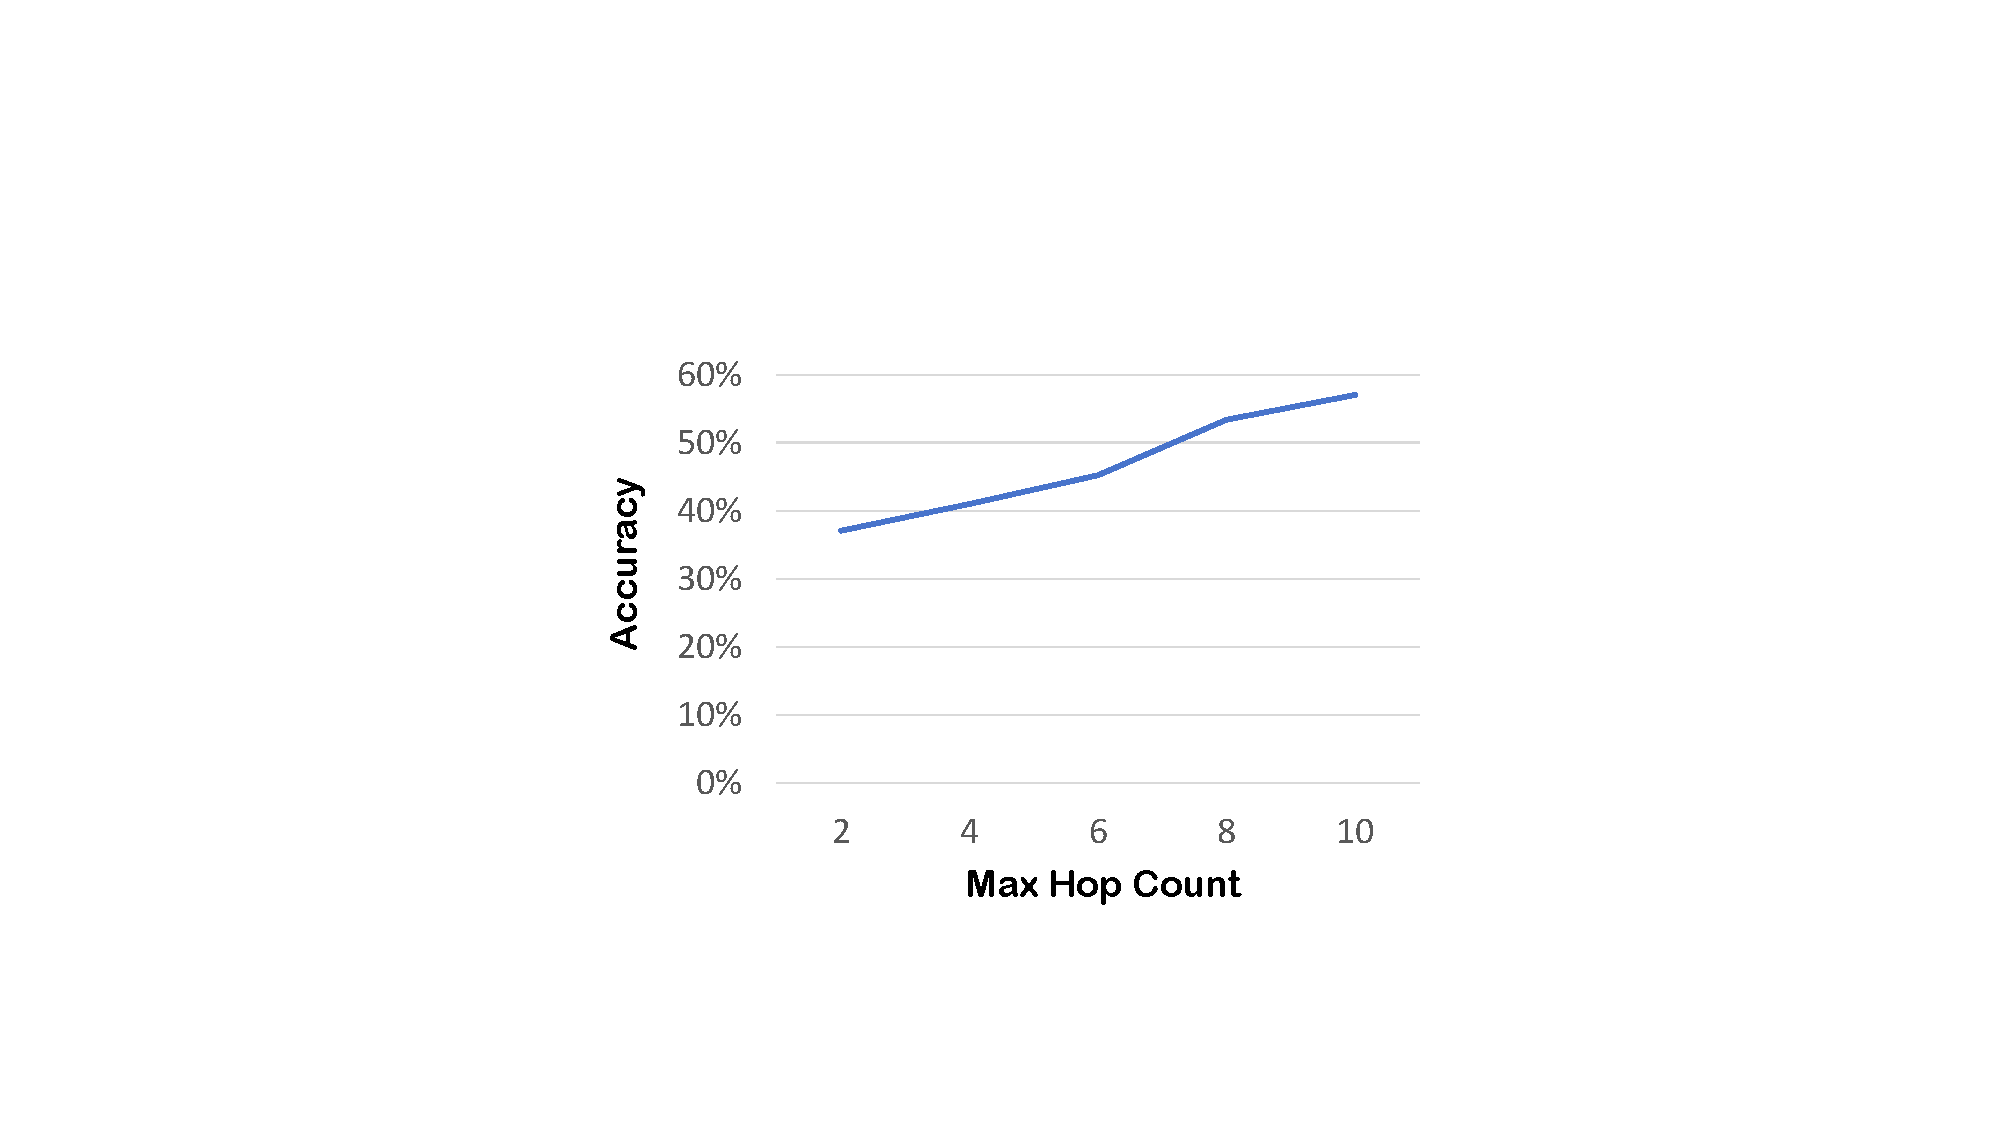
\includegraphics[width=\linewidth]{Resources/Impact_of_Hop_Count_1.pdf}
        \caption{Performance on Long Dependency QA.}
    \end{subfigure}
    \hfill
    \begin{subfigure}[b]{0.48\textwidth}
        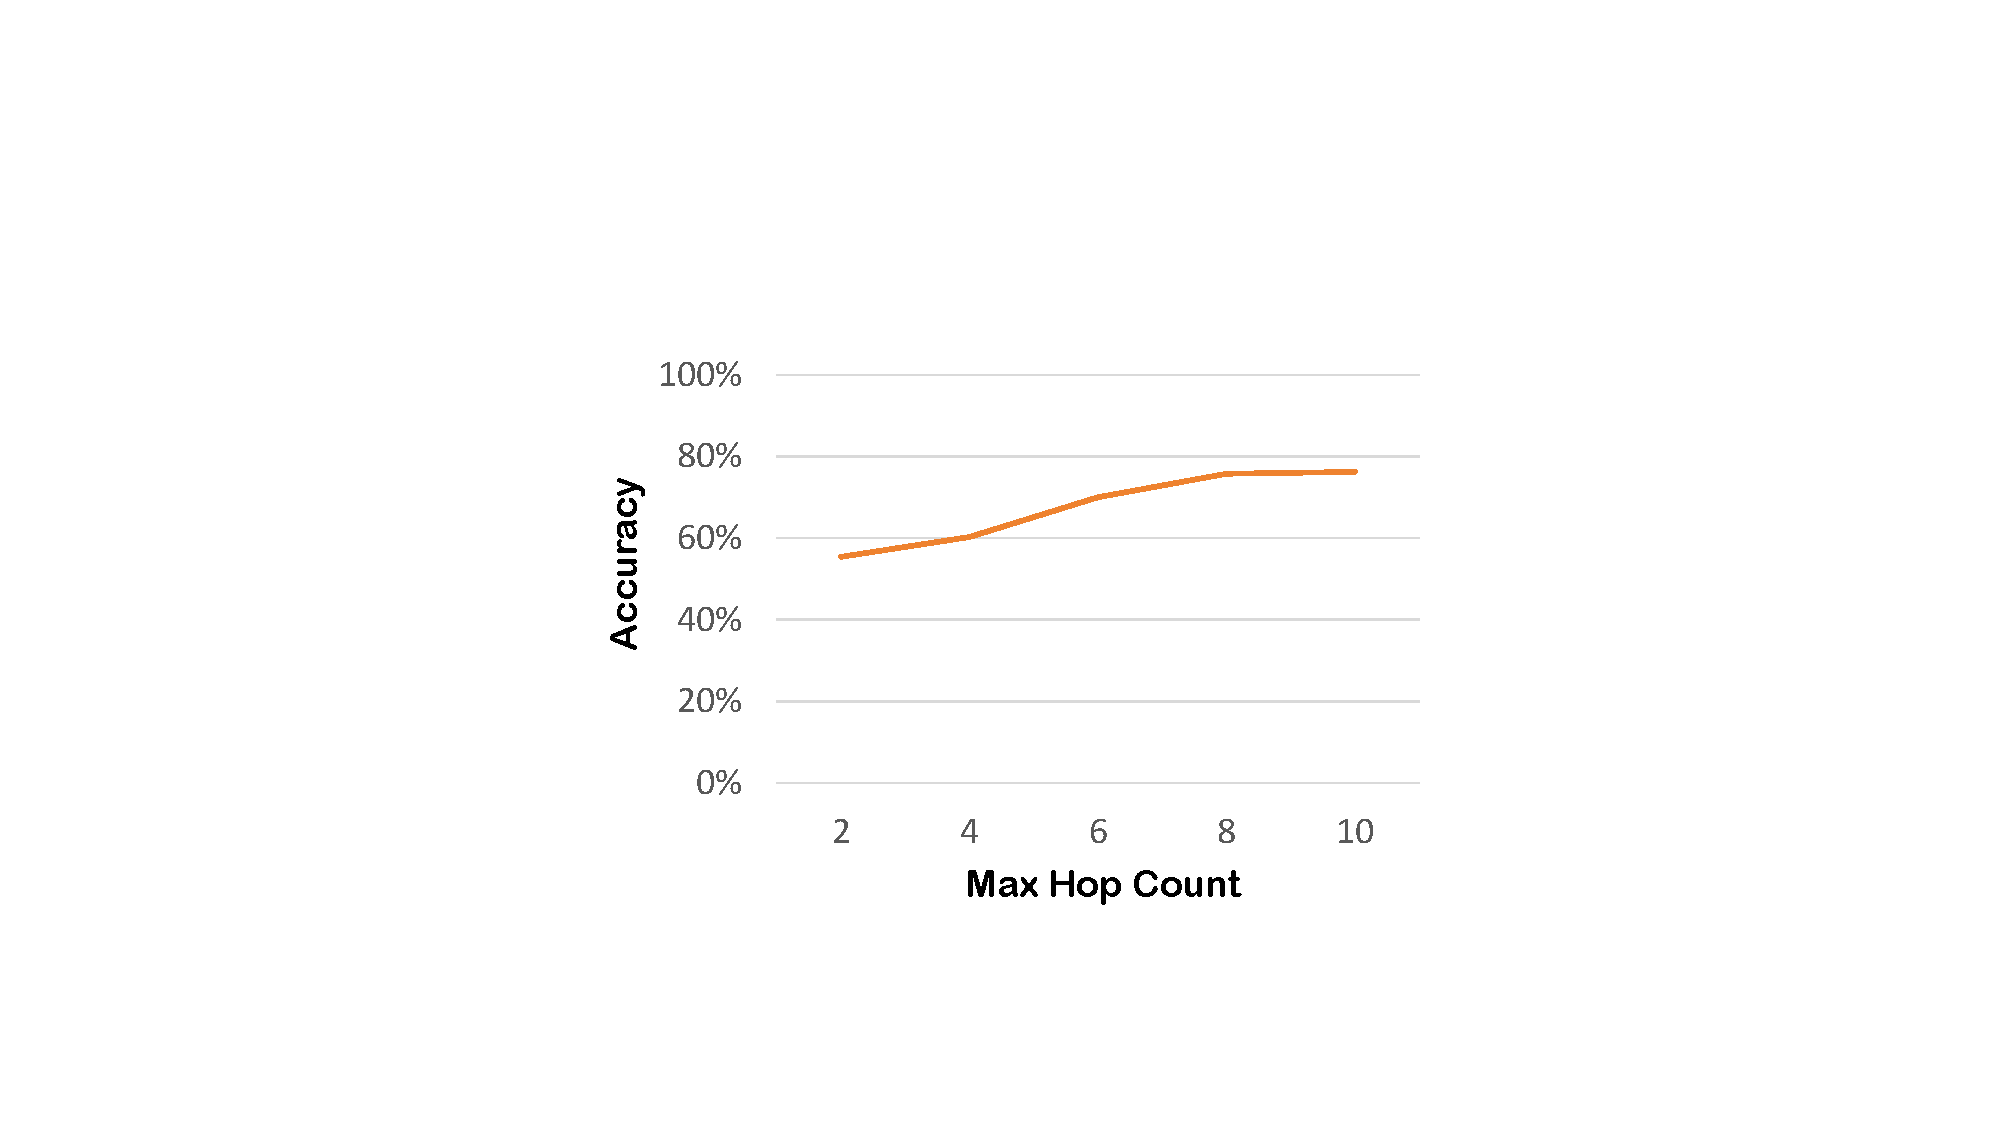
\includegraphics[width=\linewidth]{Resources/Impact_of_Hop_Count_2.pdf}
        \caption{Performance on Multi-Hop QA.}
    \end{subfigure}
    \caption{The Impact of Different Hop Count Settings.}
    \label{fig:hop-count}
\end{figure}


\begin{wraptable}{r}{0.7\textwidth}
    \begin{tabular}{l|c|c|c}
        \toprule
        Methods & Avg. API Calls & Token Ratio & Total Tokens \\
        \midrule
        \midrule
        \ours & 2 & 2.64 & 1.25M\\
        \midrule
        GraphRAG \cite{Main3} & 14.73 & 15.42 & 7.31M\\
        HippoRag2 \cite{Main6} & 2 & 3.91 & 1.87M\\
        \bottomrule
    \end{tabular}
    \caption{Graph Building Comparative Experiment.}
    \label{fig:graph-build-compare}
\end{wraptable}

\textbf{The Impact of Different Hop Count Settings.} We investigate the influence of various hop count configurations on system performance. Specifically, through experiments, we analyze the effect of the Maximum Hop Count parameter in the \ours~ model (the relevant parameter definitions are detailed in \Cref{appendix:parameter-configuration}). As illustrated in \Cref{fig:hop-count}, the experimental results demonstrate a significant positive correlation between model performance and hop count settings: as the Maximum Hop Count value increases, the classification accuracy of the system exhibits a monotonically increasing trend. This finding aligns with the fundamental principle of the LLM-Guided Knowledge Graph Traversal in \ours, where a larger hop count enables nodes to access broader neighborhood information, thereby enhancing their information-gathering capability.


\textbf{Cost Analysis of Graph Building.} We compare the graph building costs between \ours~ and other baselines. As shown in \Cref{fig:graph-build-compare}, experimental results on the LooGLE dataset demonstrate that our method achieves a significantly lower ratio of consumed tokens to source text tokens during the construction process compared to high-overhead systems like GraphRAG\cite{Base3}, while maintaining competitive performance against other baseline approaches.


\textbf{Analysis on Path Consistency}. To demonstrate that semantically similar queries correspond to similar graph paths, we design an experiment to quantify the similarity between search paths of an original problem and a similar problem. We model the search paths as sets of \textit{edges}, where an "edge" refers to a direct connection between two nodes. Let \( E_1 \) represent the set of edges in the original problem's search path, and \( E_2 \) represent the set of edges in the similar problem's search path.

The similarity \( S \) between \( E_1 \) and \( E_2 \) is defined as the ratio of the number of identical edges (intersection of the two sets) to the total number of unique edges (union of the two sets after deduplication). Formally, this is expressed as:
\[
S = \frac{|E_1 \cap E_2|}{|E_1 \cup E_2|}
\]
Here, \( |E_1 \cap E_2| \) denotes the cardinality of the intersection (i.e., the count of edges shared by both search paths), and \( |E_1 \cup E_2| \) denotes the cardinality of the union (i.e., the total count of distinct edges present in either search path). A \( S \) value closer to \( 1 \) indicates a higher overlap between the two search paths (implying more similar underlying logic), while a value closer to \( 0 \) indicates greater divergence.

To obtain a comprehensive measure, we define the aggregated similarity \( S_{\text{avg}} \) as the average of all individual similarity values from multiple calculations:
\[S_{\text{avg}} = \frac{1}{n} \sum_{i=1}^{n} S_i\]
where \( n \) is the total number of similarity calculations performed, and \( S_i \) is the similarity from the \( i \)-th calculation. We first ran the original problems and then the corresponding similar problems. Taking the base model GPT-4o-mini as an example, the experimental results for similarity are presented in Table \ref{tab:similarity-result}. From these experimental results, it is evident that semantically similar queries induce similar graph paths.

\begin{table}[ht]
\captionsetup{skip=10pt} 
\centering
\begin{tabular}{l|c}
\toprule
Task               & \( S_{\text{avg}} \) \\
\midrule
LongDependencyQA   & 53.78\% \\
\bottomrule
\end{tabular}
\caption{Similarity results for the base model GPT-4o-mini.}
\label{tab:similarity-result}
\end{table}



\textbf{Query Order Impact}. To evaluate whether the order of questions (introduced via random shuffling) affects the system's performance, we designed an experiment where questions in the dataset were randomly shuffled \textit{before each system update}, with three accuracy measurements taken to assess the system's robustness to input order variations.

Specifically, we integrated a random question shuffling module into our codebase. The experiment proceeded in three stages: 
- For \textit{Update times = 0}: We first randomly shuffled the questions and measured the system's accuracy without any prior updates;
- For \textit{Update times = 1}: After the first system update, we re-randomly shuffled the questions (generating a new order distinct from the first) and measured accuracy;
- For \textit{Update times = 2}: After the second system update, we again re-randomly shuffled the questions (generating a third unique order) and measured accuracy.

For each stage, we also recorded the \textit{original accuracy} (i.e., accuracy with unshuffled questions) for comparison. The experimental results are summarized in Table \ref{tab:shuffling-impact}.

\begin{table}[ht]
\captionsetup{skip=10pt}
\centering
\begin{tabular}{l|c|c}
\toprule
Update times & Accuracy (With Re-shuffled Questions) & Original Accuracy (Unshuffled) \\
\midrule
0            & 56.37\%                               & 57.04\%                         \\
1            & 55.78\%                               & 56.48\%                         \\
2            & 57.71\%                               & 58.01\%                         \\
\bottomrule
\end{tabular}
\caption{System accuracy on Long-Dependency-Task with re-randomized question orders before each update (with original accuracy for comparison). A new shuffled order was used for each update stage. }
\label{tab:shuffling-impact}
\end{table}

From Table \ref{tab:shuffling-impact}, we observe that even with a fresh random shuffle of questions before each update, the system's accuracy remains consistently close to the original accuracy (with unshuffled questions) across all stages. Specifically, at \(\text{Update times} = 0\), the shuffled accuracy (\(56.37\%\)) is comparable to the original (\(57.04\%\)); after the first re-shuffle and update (\(\text{Update times} = 1\)), the gap remains minimal (\(55.78\%\) vs. \(56.48\%\)); and after the second re-shuffle and update (\(\text{Update times} = 2\)), the trend persists (\(57.71\%\) vs. \(58.01\%\)). These results confirm that repeated random shuffling of question order—even before each system update—has negligible impact on performance, demonstrating the system's strong robustness to input order variations.


\subsection{Additional Analysis on Baselines}
\label{appendix::supplementary-experimental-details}


\subsubsection{Analysis of PoG}
\label{appendix:::some-details-of-PoG}
In the field of KGQA (Knowledge Graph Question Answering), we select the latest method PoG (a self-correcting adaptive planning paradigm for KG-augmented LLMs) as a representative. Since the original method is exclusively designed for the Freebase knowledge graph \cite{freebase}, we modify the source code of PoG (the revised code is open-sourced on GitHub) to adapt it to our own knowledge graphs, allowing traversal of nodes in our constructed knowledge graphs. (As PoG only handles node-level processing, the knowledge graph provided to PoG excludes the chunk component.) We greatly appreciate their open-source contribution.

\begin{wraptable}{r}{0.6\textwidth} 
\centering
\begin{tabular}{l|c|c}
\toprule
\textbf{QA Type} & \textbf{GPT-4o-mini} & \textbf{DeepSeek-V3} \\ 
\midrule
Long Dependency QA & 30.29K & 25.88K \\
Multi-Hop QA       & 5.53K & 6.96K \\
Simple QA          & 27.11K & 21.21K \\
\bottomrule
\end{tabular}
\vspace{0.5em} 
\caption{Comparison of the Average Token Consumption of the PoG Method across Different QA Types}
\label{tab:token_consumption}
\end{wraptable}

We retain PoG's implementation methodology and prompts, only altering the output examples in parts of the prompts to adapt to the format; code differences can be viewed at \url{https://anonymous.4open.science/r/PoG_adapted-C5C0.} The accuracy rates show that the method of conducting Large Language Model (LLM) traversal search solely on the nodes of the knowledge graph, which lacks all textual information, significantly reduces the search accuracy. Compared with our method, PoG’s performance on each dataset drops significantly.

Additionally, DeepSeek-V3 exhibits a more pronounced inclination toward a conservative strategy, leading to a higher search depth and greater token consumption compared to GPT-4o-mini. It frequently outputs null answers due to perceived lack of sufficient information, which is also clearly evident in GraphRAG (\Cref{appendix:::abnormal-results-of-GraphRAG}).

Since the source code of PoG mentions that the maximum search depth is set to 4, in the case of a knowledge graph relying on long-text associations (the revised code we wrote sets the maximum depth to 10, which is consistent with our method), the performance is poor, and the consumption of tokens has significantly increased compared with ours, as shown in \Cref{tab:token_consumption}. However, for the simple multi-hop dataset of HotPotQA, which extracts information from Wikipedia and has extremely limited information volume, token consumption is more optimized than ours. We believe that such a simple question-answering dataset cannot well represent the real-world scenarios, and many questions still require complex information extraction. Therefore, the efficiency optimization of searching in complex datasets is of greater application value.
For other methods, since they do not involve LLM traversal, comparing token consumption is of little significance.

\subsubsection{Analysis of GraphRAG}
\label{appendix:::abnormal-results-of-GraphRAG}
Based on the feedback on similar issues from GitHub users, we hereby analyze the reasons for the relatively poor performance of GraphRAG\footnote{\url{https://github.com/microsoft/graphrag/issues/682}}.In order to aim for a low hallucination rate, GraphRAG often outputs responses like "More information is needed." For example, \Cref{fig:deepseek-problem} shows a question and its generated answer.


\begin{figure}[h]
    \centering
    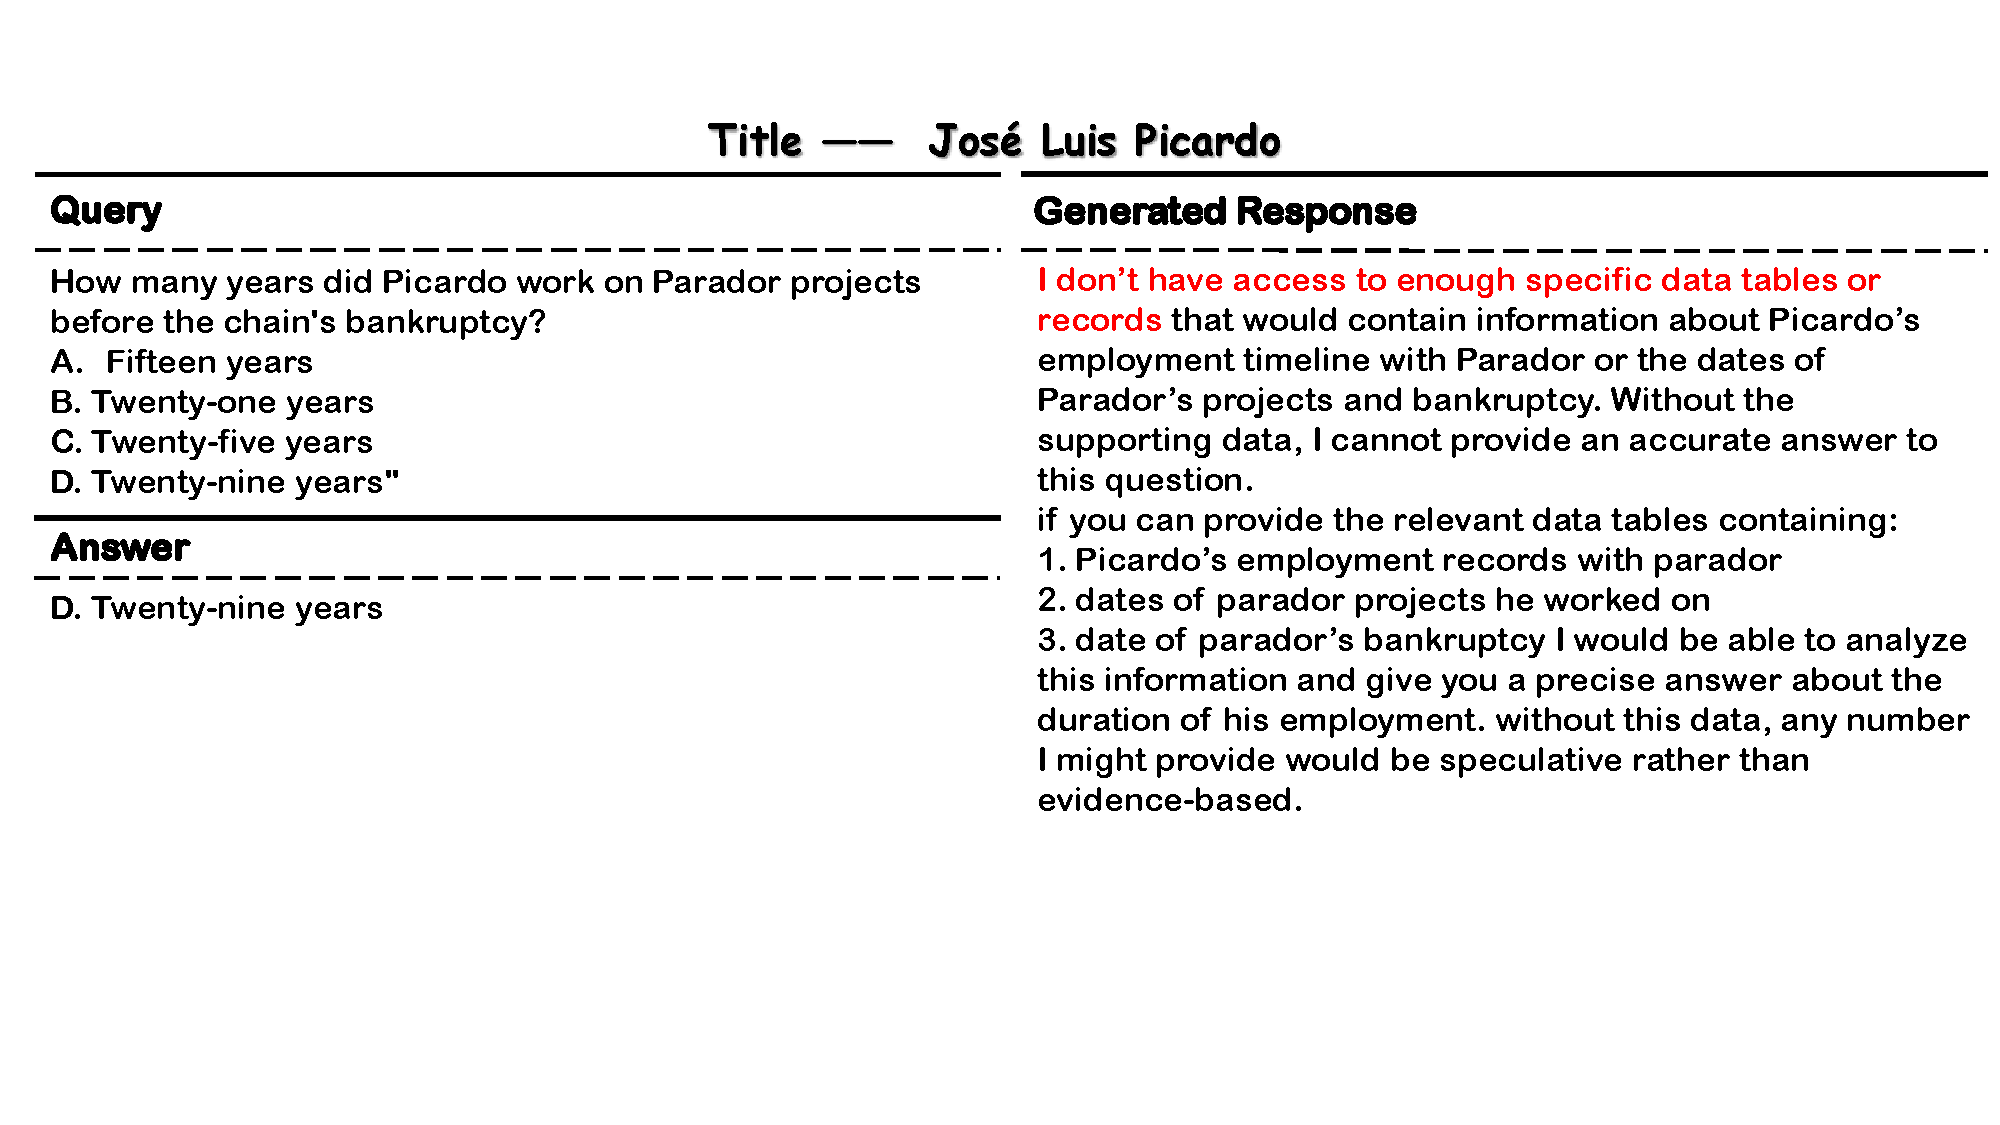
\includegraphics[width=1\textwidth]{Resources/graphrag_experiment_result.pdf}
    \caption{Comparative Illustration of Subtle Difference Questions in the Knowledge Graph.}
    \label{fig:deepseek-problem}
\end{figure}

Deepseek-V3 is more inclined to provide conservative outputs compared to GPT-4o-mini (often requesting more information from users instead of providing direct answers), so its accuracy rate has dropped significantly. We have also found that, unlike other methods, GraphRAG is more effective at retrieving for long-dependency question-answering tasks, while its retrieval ability for short-dependency question-answering tasks has declined.


